\chapter{Конструкторский раздел}
В этом разделе будут приведены требования к ПО, схемы реализации алгоритмов,
а также выбранные классы эквивалентности для тестирования ПО.

\section{Требования к ПО}
Ниже будет представлен список требований к разрабатываемому программному обеспечению. 

Требования к входным данным: 
\begin{itemize}
	\item на вход подаётся массив, состоящий из вещественных чисел;
	\item в массиве минимум два элемента;
	\item в массиве минимум два элемента отличаются друг от друга.
\end{itemize}

Требования к выводу: 
\begin{itemize}
	\item программа должна вывести логи обработки данных при выполнении различных заданий.
\end{itemize}

\section{Схемы алгоритмов}
На рисунке 2.1 будет приведена схема реализации линейного алгоритма стандартизации данных.

На рисунках 2.2-2.5 будут приведены схемы реализации алгоритма стандартизации данных с использованием конвейерных вычислений.

\FloatBarrier
\begin{figure}[hp]
	\label{classic}
	\begin{center}
		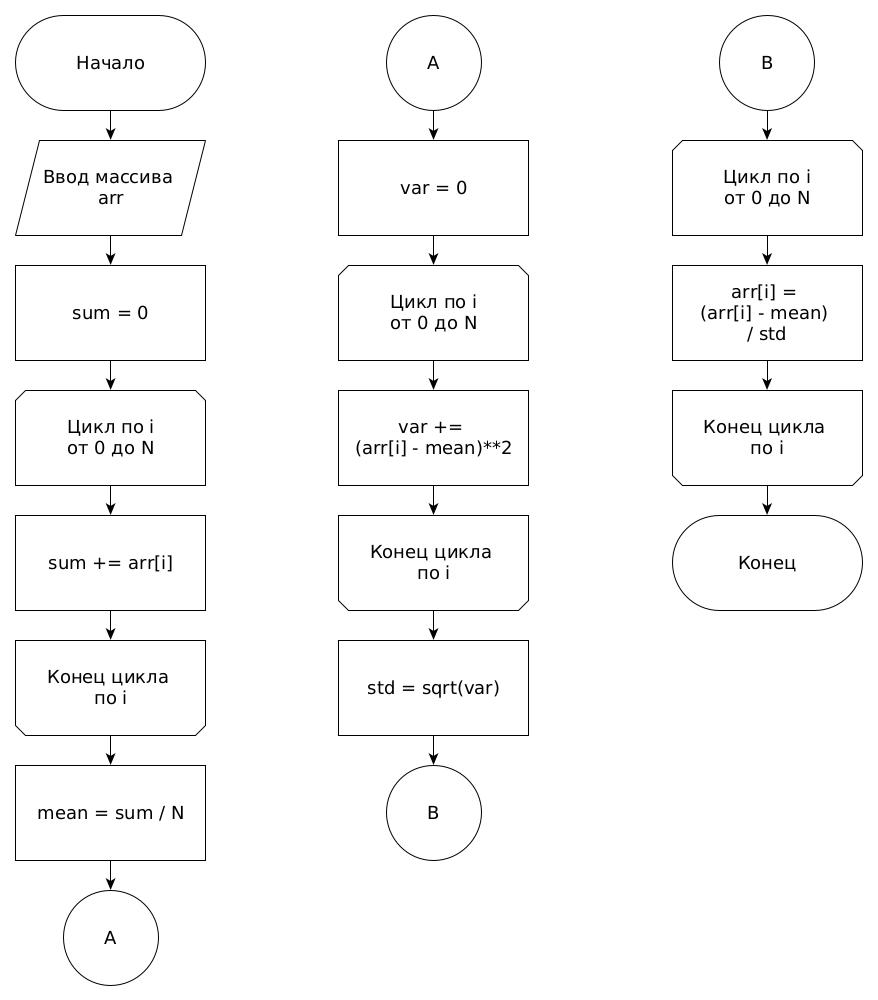
\includegraphics[width=\linewidth]{graph/classic.jpg}
	\end{center}
	\caption{Схема линейного алгоритма стандартизации данных}
\end{figure}
\FloatBarrier

\FloatBarrier
\begin{figure}[hp]
	\label{classic}
	\begin{center}
		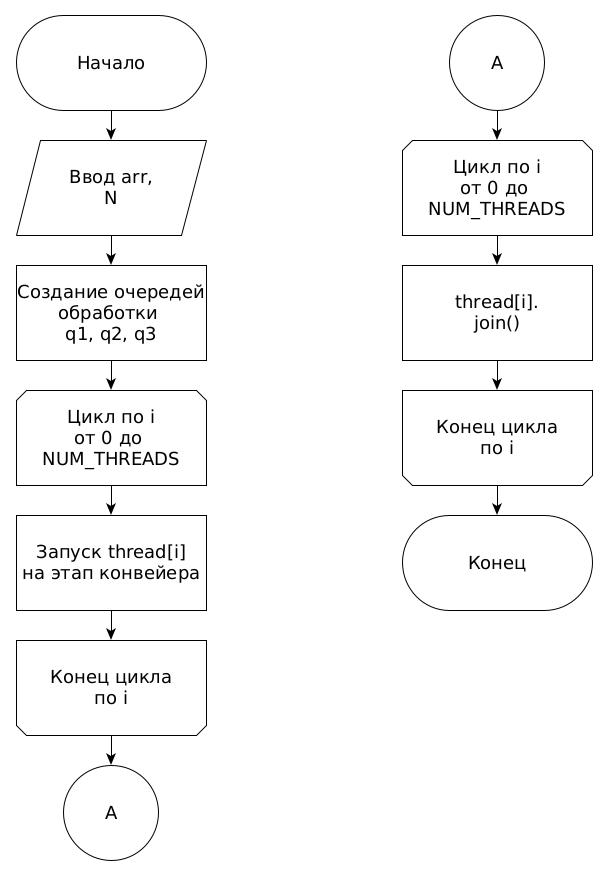
\includegraphics[width=\linewidth]{graph/paral.jpg}
	\end{center}
	\caption{Схема работы главного потока для реализации алгоритма стандартизации данных с использованием конвейера}
\end{figure}
\FloatBarrier

\FloatBarrier
\begin{figure}[hp]
	\label{classic}
	\begin{center}
		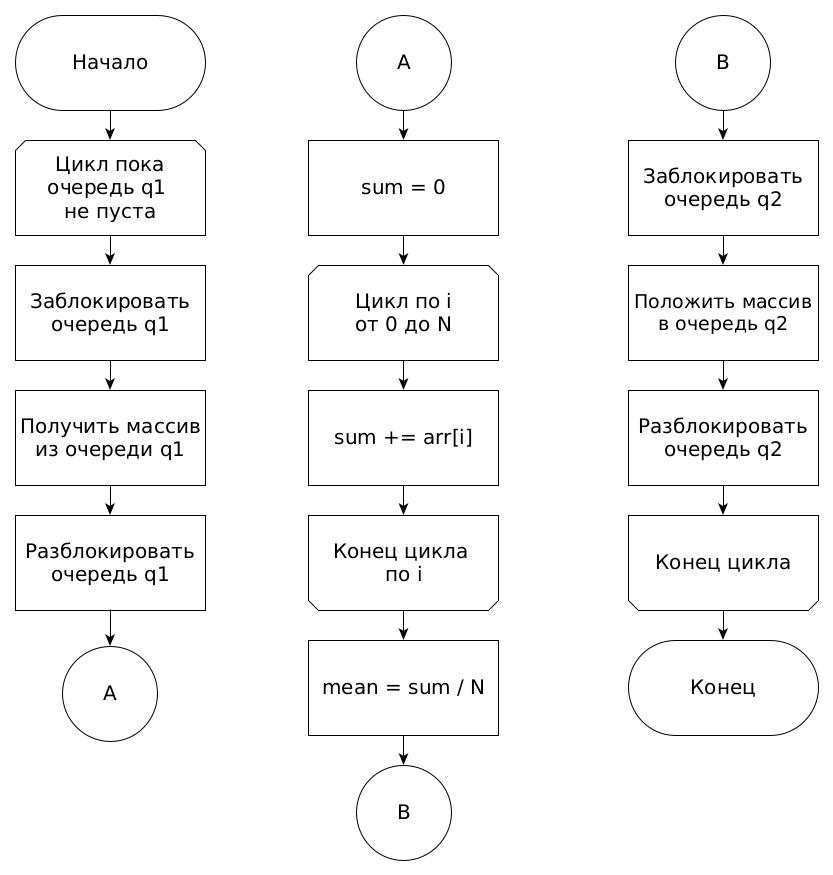
\includegraphics[width=\linewidth]{graph/ex1.jpg}
	\end{center}
	\caption{Схема работы потока на первом этапе конвейерных вычислений}
\end{figure}
\FloatBarrier

\FloatBarrier
\begin{figure}[hp]
	\label{classic}
	\begin{center}
		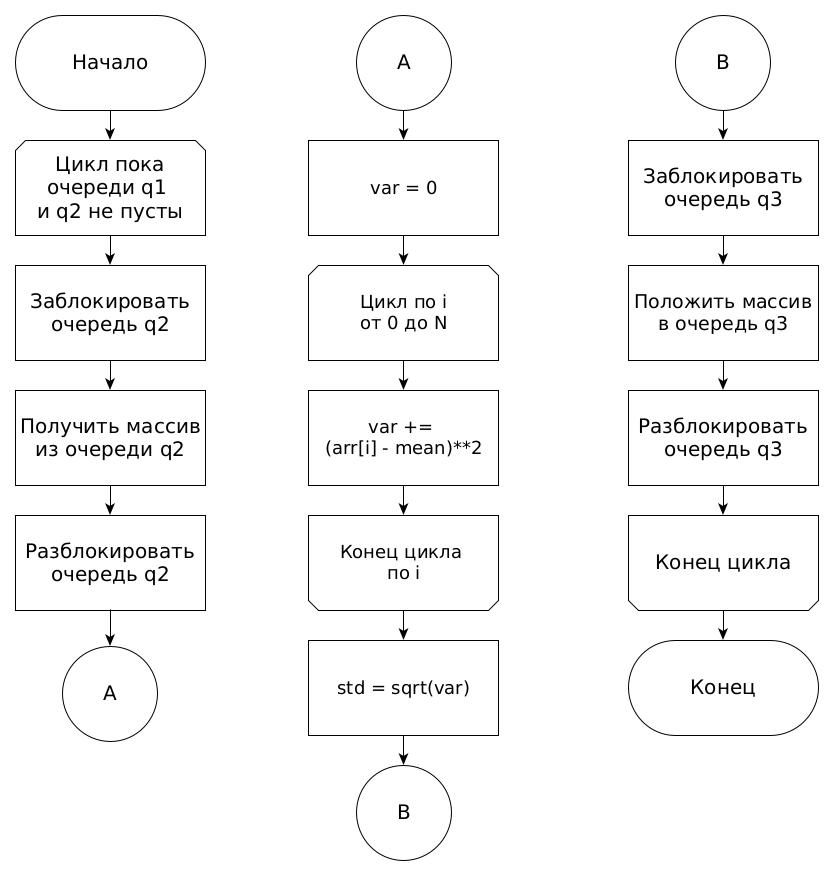
\includegraphics[width=\linewidth]{graph/ex2.jpg}
	\end{center}
	\caption{Схема работы потока на втором этапе конвейерных вычислений}
\end{figure}
\FloatBarrier

\FloatBarrier
\begin{figure}[hp]
	\label{classic}
	\begin{center}
		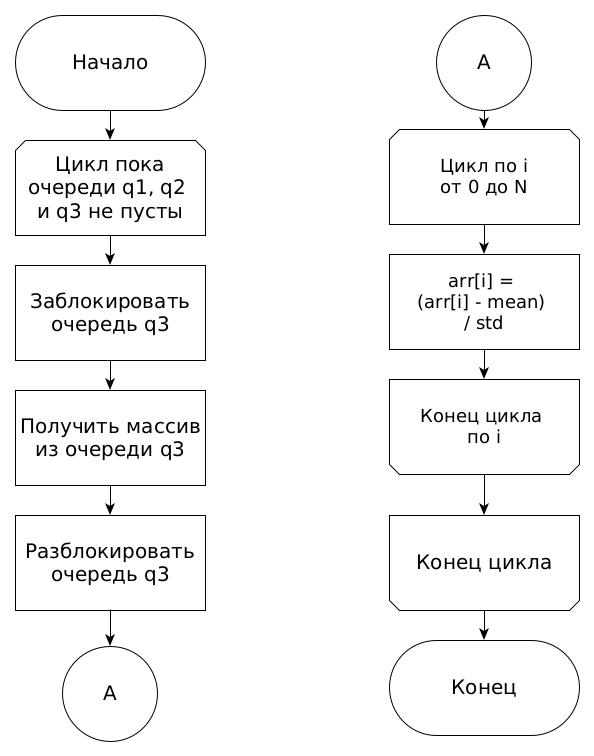
\includegraphics[width=\linewidth]{graph/ex3.jpg}
	\end{center}
	\caption{Схема работы потока на третьем этапе конвейерных вычислений}
\end{figure}
\FloatBarrier


\section{Типы данных для алгоритмов}
Тестирование алгоритмов будет производиться на вещественных числах, 
которые могут быть и отрицательными, и равны нулю. Несмотря на это,
сами реализации алгоритмов универсальны и предназначены для любых численных типов данных.

Размер массива может быть произвольным из тех, что допустимы по требованиям ко вводу.

\section{Способ тестирования}
Тестирование программы будет произодиться методом чёрного ящика.
Такой подход выбран, так как от реализаций алгоритмов требуется в первую
очередь правильность работы.
Сама по себе реализация не требует тестировки, так как в точности
повторяет теоретические принципы, сформированные в аналитическом
разделе.

В качестве классов эквивалентности были выбраны следующие сущности:
\begin{itemize}
	\item массив состоит из двух элементов;
	\item массив состоит из множества разных элементов;
	\item массив состоит из целых чисел, следующих на числовой прямой друг за другом (например, -1 0 1).
	\item массив состоит из чисел, очень близких друг к другу.
	\item массив состоит из 5 чисел от 0 до 1000
\end{itemize}

Для тестирования требуется сравнить полученное значение с эталонным.
Для этого использовалась библиотека Sklearn и метод StandartScaler, который
выполняют стандартизацию входного массива.

\section{Вывод}
Были приведены требования к ПО, схемы реализации алгоритмов.
Был определен способ тестирования алгоритмов.